\section{Theory}

Usually, when designing digital circuits, two major simplifications
are made. The first is that the signals are discrete, or digital. The
second simplification is to look at the time as discrete. Theese
simplifications makes it meaningful to talk about momentarily state of
the circuits, namely the contents of memory elements. The concept of
next state is also meaningful, as the whole circuit is synchronized by
a common clock, which also assures correct timing and data validity
across the circuit.

When designing clockless circuits, the second simplification no longer
holds. Technical aspects, like timing and data validity, must be
guaranteed by other means. For the designer, it demands a change in
the reasoning, as it is, in general, no longer meaningful to look at a
momentarily state.

In this section, I will discuss the technical aspects of clockless
design, while design tools for designing will be discussed in
section~\ref{sec:tools}.

The strictest class of clockless circuits, delay insensive (DI)
circuits, assumes only bounded and positive, but unknown, delays in
wires and gates. Such circuits can only be constructed of C-elements
(see Figure~\ref{fig:c}) and inverters. In \cite{dilimit} it is shown
that it is impossible to create any useful circuits with this
methodology. The article suggests the introduction of a timing
assumption to facilitate the construction of useful circuits: The
isochronic fork.

\begin{figure}[htbp]
  \centering
  \includegraphics{c.pdf}
  \caption{a) Symbol for a Muller C-element. b) Karnough-map c)
    Gate-level implementation}
  \label{fig:c}
\end{figure}

An isochronic fork is a timing assumption that requires a signal to be
delivered simultainiously to two circuit elements. This fork allows
the sender of a signal to assume reception with only one acknowledge
signal. The class of circuits depending on isochronic forks are said
to be quasi delay insensitive (QDI), and it is also turing complete
\cite{turing}, meaning that useful circuits can be designed in this
methodology.

Speed insensitivity.

Handshake circuits.

When designing clockless circuits, we need a substitute for the clock
to assure data validity, and flow for the memory elements. This is
done with handshaking, usually implemented with a request-acknowledge
protocol as shown in figure~\ref{fig:hanshake}. The handshaking
provides a local clock for the storage elements\footnote{Usually
  single latches, as master-slave latches is unneeded.}.

There are multiple ways to implement handshaking. This project will
focus on high-level synthesis that is agnostic on the underlying
protocol (it can even be clocked). 

\subsection{2-phase and 4-phase handshaking}


\subsection{Push and pull channels}

\subsection{Indication and the muller-C element}

\subsection{Bundled-data}

When using bundled-data, values are represented by conventional
boolean levels, and the handshaking is implemented by bundeling the
request and acknowledge signals with the data as shown in
figure~\ref{fig:bundeled}. Bundled data is also refered to as
single-rail.

As binary data usually has no way of indicating completion, matching
delays has to be inserted to maintain correct behaviour as shown in
figure~\ref{fig:bundeled_delay}.

\subsection{Dual rail}

If the signal is encoded into a representation using two wires per
bit, one for each value; logic 1 (true) and logic 0 (false). This
redundant representation provides the possibility of a variable to
have an ``empty'' value. 

By carefully designing the combinational blocks without hazards, it is
possible to detect when values are completely computed. An example of
a circuit for completion detection is shown in figure
\ref{fig:completion}. By using this completion-detection for the
request (or acknowledge) signal, the circuit can be made delay
insensitive.

\subsection{Summary}


%\begin{quote}
%A register may input and store a new data token from its predecessor
%if its successor has input and stored the data token that the register
%was previously holding
%\end{quote}

